\problemname{Kubiska boxar}
Din syssling Paulo R älskar boxar.
Just nu är du på väg att fira jul hos Paulo (traditionsenligt firar du jul en gång med varje del av din släkt, som just nu består av 72 olika familjer).
Tyvärr har du precis insett att du glömt att köpa julklappar!

Eftersom Paulo älskar boxar, är detta precis vad du tänker köpa till honom.
En box är kubisk med en viss sidlängd, och har en av tre färger -- röd (R), grön (G) eller blå (B).
Du har skrivit ner en inköpslista med alla boxar du tänker köpa.
Tyvärr säljs boxarna i tre olika butiker, där varje butik säljer boxar av en viss färg.

Din plan är nu att åka till alla tre butiker för att köpa de nödvändiga boxarna.
För att spara plats i baggageutrymmet tänker du placera vissa av boxarna i varandra.
Om du besöker butikerna i ordningen $f_1, f_2, f_3$, (t.ex. R, G, B) så får du placera boxar av färgen $f_3$ i boxar av färgen $f_2$, och boxar av färgen $f_2$ i boxar av färgen $f_1$.
Ordningen R, G, B innebär alltså att Paulo kan placera blåa boxar i gröna boxar, och gröna boxar i röda boxar.
Du får \textbf{inte} placera boxar av färgen $f_3$ i boxar av färgen $f_1$ -- det hade ju varit helt absurt.
Dessutom kan en box bara placeras i en box som har en \textbf{strikt större} sidlängd.

\begin{figure}[h!]
  \centering
  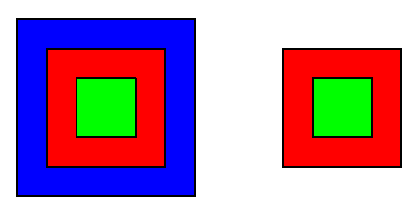
\includegraphics[width=0.5\textwidth]{sample3}
  \caption{En möjlig lösning till exempel 3.
  Till vänster en grön box är placerad i en röd box som är placerad i en blå box.
  Till höger en grön box placerad i en röd box.}
  \label{fig:sample3}
\end{figure}

Kan du avgöra i vilken ordning du ska besöka butikerna, för att minimera antalet \emph{ytterboxar} (d.v.s. boxar som inte ligger inuti en annan box), om du placerar boxarna optimalt?

\section*{Indata}
Indatan börjar med talet $N$, antalet boxar, där $1\le N \le 1\,000$. Därefter följer $N$ rader med sidlängd
$l_i$ ($1 \le l_i \le 10\,000\,000$) och färg $f_i$ (R, G, eller B) för varje box.

\section*{Utdata}
Du ska skriva ut två rader.
Den första raden ska innehålla den ordning du besöker butikerna i, på formen $f_1\text{ }f_2\text{ }f_3$.
Den andra raden ska bestå av ett heltal -- det minsta antalet ytterboxar du kan åstadkomma efter att du stoppat in boxarna i varandra.

\section*{Poängsättning}
Din lösning kommer att testas på en mängd testfallsgrupper. För att få poäng för en grupp
så måste du klara alla testfall i gruppen.

\noindent
\begin{tabular}{| l | l | l |}
\hline
% Grupp & Poängvärde & Gränser & Övrigt \\ \hline
Grupp & Poängvärde & Gränser \\ \hline
1     & 50         & Du kommer alltid besöka butikerna i ordningen \texttt{B G R} \\ \hline
2     & 50         & Inga begränsningar. \\ \hline
\end{tabular}

\section*{Förklaring av exempel 3}
En möjlig lösning är illustrerad i Figur~\ref{fig:sample3}.
Den optimala ordningen är att besöka butikerna i ordningen blå, röd, grön.

Vi kan då lägga de två G-boxarna (storlek 1) i varsin R-box (storlek 10).
Därefter kan den ena R-boxen läggas i en B-box.
Kvar återstår då en R-box och en B-box som ytterboxar.
